\documentclass[11pt]{article}
\usepackage[margin=1in]{geometry}
\usepackage{amsmath,amssymb,amsthm}
\usepackage{graphicx}
\usepackage{xcolor}
\usepackage[colorlinks=true,linkcolor=blue,citecolor=blue,urlcolor=blue]{hyperref}

\newtheorem{prop}{Proposition}
\newcommand{\dd}{\mathrm{d}}
\newcommand{\E}{\mathbb{E}}
\newcommand{\Prob}{\mathbb{P}}

\title{\textbf{Step 0: why the leader always falls}\\[2pt]
\large rise-and-fall in the pure-growth model, derived}
\author{M.\ Heltberg}
\date{Stepwise-progression note, June 2026}

\begin{document}
\maketitle

\noindent\emph{Folder \texttt{stepwise\_progression/}. Code: \texttt{step0\_growth.py}
(base model), \texttt{step0\_turnover.py} (the measurements and figure below).}

\begin{abstract}
\noindent The base model has no wars, alliances, or decisions --- only
resource-limited growth of $N$ states. Empirically a single state dominates for a
while and is then \emph{always} overtaken: the condensate is dynamic. We show this
analytically. Once the shared resource is exhausted the strength of any state, in
particular the leader, obeys a driftless equation $\dd S=\sigma\sqrt S\,\dd W$,
which after $S\mapsto 2\sqrt S$ is a Bessel process of dimension $0$
(equivalently $S$ is a squared-Bessel \textsc{besq}$(0)$). Such a process is a
nonnegative martingale that reaches $0$ almost surely; optional stopping gives the
sharp statement that, from its current size $S_0$, the leader reaches a level
$a>S_0$ before collapsing only with probability $S_0/a$. Permanent dominance is
therefore impossible. We also identify the structural cause --- \emph{additive}
(size-independent) growth, whose drift-to-noise ratio falls as $S^{-1/2}$ --- and
contrast it with multiplicative growth, which locks in.
\end{abstract}

% ====================================================================
\section{Model}

$N$ states with strengths $S_i\ge0$ and growth rates $\gamma_i$. The only coupling
is the global resource availability $R$:
\begin{align}
R(t)&=\max\!\Big(1-\tfrac1K\textstyle\sum_j S_j,\,0\Big),\label{eq:R}\\
\dd S_i&=\gamma_i\,R\;\dd t+\sigma\sqrt{S_i}\,\dd W_i,\label{eq:S}\\
\dd \gamma_i&=\lambda_g(\mu_g-\gamma_i)\,\dd t+\sigma_g\,\dd W^g_i.\label{eq:g}
\end{align}
Two features matter below: the growth drift $\gamma_i R$ is \emph{additive}
(independent of $S_i$), and the noise is \emph{demographic}, of amplitude
$\sigma\sqrt{S_i}$ (Itô; $\sigma=\texttt{sig\_s}$). Defaults: $N=10$, $K=10N$,
$\sigma=1$.

% ====================================================================
\section{The phenomenon}

Measured over a run of length $t=200$ (Fig.~\ref{fig:turn}a): the instantaneous
leader $\arg\max_i S_i$ changes $\sim 55$--$65$ times, $6$--$10$ distinct states
hold the lead, and the leader at mid-run is still leading at the end only
$\approx42\%$ of the time. No state stays on top.

\begin{figure}[h]
\centering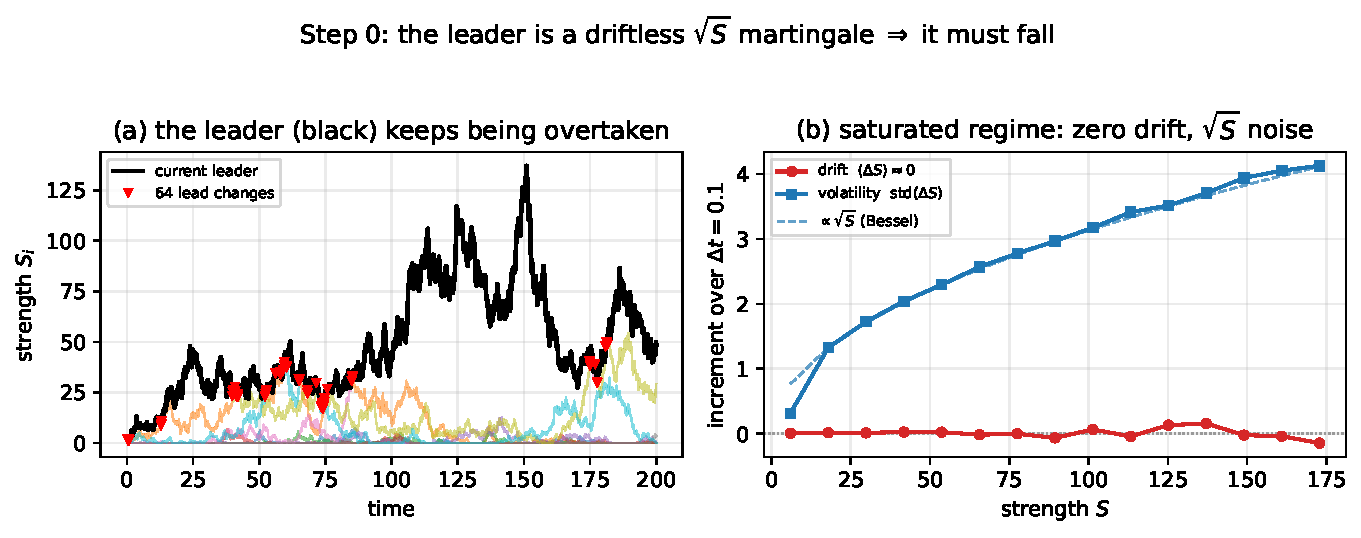
\includegraphics[width=\textwidth]{figs/step0_turnover.pdf}
\caption{(a) One run: the instantaneous leader (black) is repeatedly overtaken
(red markers). (b) Pooled over $40$ runs in the saturated window $t>70$: the
conditional drift $\langle\Delta S\rangle$ is $\approx0$ at every size (red),
while the conditional volatility grows as $\sqrt S$ (blue, with the
$\propto\sqrt S$ guide). This is the signature of the driftless $\sqrt S$
martingale derived in \S\ref{sec:bessel}.}
\label{fig:turn}
\end{figure}

% ====================================================================
\section{Saturation: the drift vanishes}\label{sec:sat}

Summing \eqref{eq:S}, the total $\Sigma=\sum_iS_i$ has drift
$R\sum_i\gamma_i$. While $R>0$ and $\sum_i\gamma_i>0$ the total grows, so $\Sigma$
rises toward $K$ and $R\downarrow0$; the resource is exhausted (in the defaults by
$t\approx70$). Once there, $R\approx0$ and \eqref{eq:S} reduces, for \emph{every}
state, to
\begin{equation}
\dd S\;\simeq\;\sigma\sqrt{S}\,\dd W .
\label{eq:driftless}
\end{equation}
The drift is then $0$ \emph{regardless of size}: this is exactly what
Fig.~\ref{fig:turn}b shows ($\langle\Delta S\rangle\approx0$ across all $S$).
Equation \eqref{eq:driftless} governs the leader.

% ====================================================================
\section{The leader is a Bessel martingale}\label{sec:bessel}

\paragraph{Martingale.} Equation \eqref{eq:driftless} has zero drift, so $S_t$ is a
(local) martingale: $\E[S_{t+s}\mid \mathcal F_t]=S_t$ as long as it has not been
absorbed. A nonnegative martingale converges almost surely; we now show the limit
is $0$.

\paragraph{Reduction to a Bessel process.} Let $Y=2\sqrt S$, so $S=Y^2/4$. With
$Y'(S)=S^{-1/2}$ and $Y''(S)=-\tfrac12 S^{-3/2}$, Itô's formula applied to
\eqref{eq:driftless}, using $(\dd S)^2=\sigma^2 S\,\dd t$, gives
\begin{equation}
\dd Y=Y'\,\dd S+\tfrac12Y''(\dd S)^2
 =S^{-1/2}\,\sigma\sqrt S\,\dd W-\tfrac14\sigma^2 S^{-1/2}\,\dd t
 =\sigma\,\dd W-\frac{\sigma^2}{2Y}\,\dd t,
\label{eq:bessel}
\end{equation}
where we used $S^{-1/2}=2/Y$. Comparing with the Bessel SDE
$\dd Y=\frac{\delta-1}{2Y}\dd t+\sigma\,\dd W$ identifies the dimension
\begin{equation}
\frac{\delta-1}{2}=-\frac12\quad\Longrightarrow\quad \boxed{\;\delta=0\;}.
\end{equation}

\paragraph{Equivalently, a squared-Bessel \textsc{besq}$(0)$.} The cleanest
statement avoids the transform. Time-change \eqref{eq:driftless} by
$s=\tfrac{\sigma^2}{4}t$ and set $B_s=\tfrac{\sigma}{2}W_t$ (a standard Brownian
motion in $s$, since $\operatorname{Var}B_s=\tfrac{\sigma^2}{4}t=s$). Then
$\sigma\sqrt S\,\dd W=2\sqrt S\,\dd B$ and \eqref{eq:driftless} becomes
\begin{equation}
\dd S=2\sqrt{S}\,\dd B=\underbrace{\delta}_{=0}\,\dd s+2\sqrt{S}\,\dd B,
\end{equation}
which is the squared-Bessel process \textsc{besq}$(\delta)$ of dimension
$\delta=0$. Standard facts: for $\delta<2$ the origin is reached almost surely,
and for $\delta\le0$ it is \emph{absorbing}. Hence

\begin{prop}\label{prop:hit}
The driftless strength \eqref{eq:driftless} reaches $0$ in finite time with
probability one. The leader is absorbed.
\end{prop}

\paragraph{How fast the lead is lost (optional stopping).} The martingale property
gives a sharp, elementary bound without invoking Bessel theory. Fix the leader's
current size $S_0$ and a target $a>S_0$, and stop at
$\tau=T_0\wedge T_a$ (first hitting of $0$ or of $a$). Since $S$ is a bounded
martingale up to $\tau$, optional stopping yields
$\E[S_\tau]=S_0$, i.e.
\begin{equation}
a\,\Prob(T_a<T_0)+0\cdot\Prob(T_0<T_a)=S_0
\;\Longrightarrow\;
\boxed{\;\Prob(\text{reach }a\text{ before }0)=\frac{S_0}{a}\;}.
\label{eq:OST}
\end{equation}
So the chance the leader ever grows to $a=2S_0,5S_0,10S_0$ before collapsing is
$\tfrac12,\tfrac15,\tfrac1{10}$; letting $a\to\infty$, $\Prob(\text{escape to }
\infty)=0$, consistent with Proposition~\ref{prop:hit}. Large further rises are
rare and collapse is generic: \emph{rise-and-fall is the typical history of every
state.} When the leader dips, $\Sigma<K$ lifts $R>0$ and the freed resource is
captured by another state, which becomes the next (temporary) leader.

% ====================================================================
\section{Why additive growth is the cause}\label{sec:additive}

The instability is specific to the \emph{additive} drift $\gamma R$. Compare the
two natural growth laws by their drift-to-noise ratio at size $S$ (drift $\mu$,
noise standard rate $\nu=\sigma\sqrt S$):
\begin{equation}
\text{additive }(\mu=\gamma R):\quad \frac{\mu}{\nu}=\frac{\gamma R}{\sigma\sqrt S}\propto S^{-1/2},
\qquad
\text{multiplicative }(\mu=\gamma R\,S):\quad \frac{\mu}{\nu}=\frac{\gamma R\sqrt S}{\sigma}\propto S^{+1/2}.
\end{equation}
For additive growth the ratio \emph{falls} as the state grows: the bigger the
leader, the more noise-dominated it is. For multiplicative growth it \emph{rises}:
large states are drift-dominated and stable. The same statement in log-strength
$y=\ln S$: by Itô, multiplicative growth gives
$\dd y=(\gamma R-\tfrac{\sigma^2}{2S})\dd t+\tfrac{\sigma}{\sqrt S}\dd W$, whose
noise $\propto S^{-1/2}\to0$ --- log-strength becomes deterministic and the leader
locks in. Empirically, replacing $\gamma R\to\gamma R\,S$ cuts the number of
leadership changes by $\sim5\times$ and makes the mid-run leader stay on top.
\emph{Additive, size-independent growth $\Rightarrow$ churn; multiplicative
$\Rightarrow$ lock-in.}

% ====================================================================
\section{A numerical caveat}

The positivity clamp \texttt{S = max(S,0)} reflects the Euler step at $0$ and
thereby injects a little strength each time \eqref{eq:S} would send $S$ negative.
Consequently $\Sigma$ is not conserved and slowly inflates above $K$ for
$t\gg200$, partly masking the \textsc{besq}$(0)$ absorption. The analysis above
concerns the clean saturated window $70\lesssim t\lesssim200$. For long-time
quantitative work use a positivity-preserving CIR scheme (full-truncation /
Alfonsi) or enforce the Feller condition $2\gamma R\ge\sigma^2$.

% ====================================================================
\section{Outlook: Step 1 (decay) should set a finite lifetime}

Turning on the decay term $-\delta S$ (defined but unused in the base code) makes
the strength a genuine \emph{CIR} process,
\begin{equation}
\dd S=\big(\gamma R-\delta S\big)\dd t+\sigma\sqrt S\,\dd W,
\end{equation}
i.e.\ mean-reverting with rate $\kappa=\delta$ toward $\theta=\gamma R/\delta$.
This is qualitatively different from \textsc{besq}$(0)$: the linear restoring
drift gives a \emph{stationary} law --- the Gamma distribution
$S_\infty\sim\Gamma\!\big(\tfrac{2\kappa\theta}{\sigma^2},\tfrac{2\kappa}{\sigma^2}\big)
=\Gamma\!\big(\tfrac{2\gamma R}{\sigma^2},\tfrac{2\delta}{\sigma^2}\big)$ --- and a
finite relaxation time $1/\kappa=1/\delta$. The Feller boundary classification
($0$ inaccessible iff $2\gamma R\ge\sigma^2$) then controls whether states can die
at all. \textbf{Prediction to test in Step~1:} decay replaces the unbounded
martingale wandering by bounded fluctuations about $\theta=\gamma R/\delta$, giving
the leader a characteristic \emph{lifetime} $\sim1/\delta$ and a tunable
rise-and-fall period, rather than the scale-free martingale collapse of Step~0.
(Note $R$ is itself dynamic: decay frees resource, so the system settles at a
total below $K$ with $R>0$ sustained, which keeps $\theta>0$.)

\end{document}
